%=====================================================================
%  DarkTrace: An Explainable, Multilingual, Forensic-Ready Dark Web
%  Threat Intelligence Framework
%
%  SCI/SCIE-style manuscript scaffold (single-column article class).
%  To port to a journal template:
%    * IEEE  : replace \documentclass with \documentclass[journal]{IEEEtran}
%    * Elsevier : \documentclass[review]{elsarticle}
%    * Springer : \documentclass{sn-jnl}
%  Compile:  pdflatex -> bibtex -> pdflatex x2
%=====================================================================
\documentclass[11pt,a4paper]{article}

\usepackage[utf8]{inputenc}
\usepackage[T1]{fontenc}
\usepackage{lmodern}
\usepackage{microtype}
\usepackage[margin=1in]{geometry}
\usepackage{amsmath,amssymb}
\usepackage{booktabs}
\usepackage{multirow}
\usepackage{array}
\usepackage{graphicx}
\usepackage{xcolor}
\usepackage{tikz}
\usetikzlibrary{shapes.geometric,arrows.meta,positioning,fit,backgrounds}
\usepackage[hidelinks]{hyperref}
\usepackage{enumitem}
\usepackage{caption}
\usepackage{authblk}

\newcommand{\framework}{\textsc{DarkTrace}}

\title{\framework{}: An Explainable, Multilingual, Forensic-Ready\\
Dark Web Threat Intelligence Framework with Severity Scoring\\
and Evidence Integrity Validation}

\author[1]{Asha Vidyadharan}
\affil[1]{\small Affiliation to be completed. Corresponding author: \texttt{codeasasha@gmail.com}}
\date{}

\begin{document}
\maketitle

%=====================================================================
\begin{abstract}
\noindent
Cyber threat intelligence (CTI) increasingly originates from the dark web, where
threat actors trade exploits, leaked credentials, and attack services across many
languages and platforms. Existing automated CTI pipelines suffer from three coupled
limitations: they are predominantly English-centric, they expose opaque
``black-box'' classifications that investigators cannot defend in operational or legal
settings, and they do not preserve the evidentiary integrity required for the outputs
to be admissible as digital evidence. We present \framework{}, an integrated framework
that unifies (i) multilingual threat classification spanning English and four
non-English languages (Hindi, Arabic, Russian, French/German), (ii) a hybrid,
explainable threat \emph{severity scoring} model whose decisions are attributed at the
token and feature level via SHAP, LIME, and transformer attention, (iii) actor and
entity extraction with STIX~2.1-aligned structuring and link analysis, and (iv) an
end-to-end \emph{forensic evidence-integrity layer} that binds every artifact to a
SHA-256 cryptographic digest, trusted timestamp, and append-only chain-of-custody
ledger. Unlike prior work that treats classification, explanation, and evidence
handling as separate concerns, \framework{} couples them so that each severity-scored,
investigator-facing alert carries both a human-readable rationale and a verifiable
provenance record. We formalize the framework, specify a reproducible dataset and
evaluation strategy over sanitized and archival dark-web corpora, define a multi-axis
metric suite (classification quality, cross-lingual transfer, explanation fidelity,
severity calibration, and tamper-evidence verification), and design a structured
ablation study isolating the contribution of each component. The paper positions the
integration of multilingual NLP, explainable severity scoring, forensic preservation,
and investigator-ready output as the core research contribution. \emph{[Replace the
following with measured results after experiments: \framework{} is expected to achieve
a macro-F1 of $\approx$0.9X on multilingual threat classification, recover $>$0.9X of
English severity ranking under zero-shot cross-lingual transfer, and provide $100\%$
tamper detection on the integrity layer.]}

\vspace{0.6em}
\noindent\textbf{Keywords:} dark web; cyber threat intelligence; multilingual NLP;
explainable AI; threat severity scoring; digital forensics; chain of custody; STIX.
\end{abstract}

%=====================================================================
\section{Introduction}\label{sec:intro}

The dark web has become a primary marketplace and discussion venue for cybercriminal
activity, hosting forums, paste sites, and hidden services through which actors trade
exploits, malware, stolen credentials, and attack-as-a-service offerings. Manual
monitoring of these sources does not scale: relevant intelligence is buried in millions
of posts, written in many languages, and is frequently obfuscated, short-lived, and
weakly labeled~\cite{schroer2025darkside,kadoguchi2019exploring}. Consequently, a
substantial body of work has applied natural language processing (NLP) and machine
learning to automate the extraction of actionable CTI from underground sources,
ranging from classical classifiers to transformer- and large-language-model-based
pipelines~\cite{sangher2023towards,sangher2024lstm,shah2025madcti,demarcos2026llm,pasupuleti2025threat}.
Recent studies report strong in-domain classification performance---for example,
BERT-based models reaching $\sim$96\% accuracy on annotated dark-web forum
content~\cite{sangher2023towards}---demonstrating that automated triage of underground
discussions is feasible.

Despite this progress, three limitations recur across the literature and, critically,
\emph{co-occur} in the operational setting that motivates this work. First, most
dark-web CTI systems are evaluated on English-only corpora, yet underground commerce is
inherently multilingual, with significant Russian-, Arabic-, and other non-English-language
activity; English-centric models degrade sharply on such content, and low-resource
languages remain systematically under-served by NLP
research~\cite{pakray2025nlp,alharbi2025bert,nazir2025multilingual}. Second, the
high-performing models deployed for threat classification are typically opaque. In
high-stakes security and forensic contexts this opacity is not a cosmetic concern: it
undermines analyst trust, hinders auditing, and weakens the defensibility of
AI-assisted findings~\cite{gaspar2024xai,hermosilla2025xai,sunkara2025xai}. Explainable
AI (XAI) methods such as SHAP and LIME have begun to be applied to intrusion detection
and CTI, but explanation is generally treated as a post-hoc add-on to a binary
detector rather than as an integral part of a calibrated, investigator-facing
\emph{severity} judgment. Third, and most neglected in the CTI-NLP literature, the
outputs of these systems are rarely produced as \emph{forensically sound evidence}.
Digital evidence is latent, volatile, and easily altered; its value in an investigation
depends on an unbroken, verifiable chain of custody and demonstrable
integrity~\cite{lone2019forensicchain,loffi2025management,patil2024potential}. A CTI
classification that cannot be tied to an immutable record of \emph{what was collected,
when, and whether it was subsequently altered} is of limited use to a law-enforcement
or incident-response investigation that may end in legal proceedings.

These three gaps are usually addressed in isolation: the multilingual NLP community
improves cross-lingual transfer~\cite{thangaraj2024crosslingual,conneau2020xlmr}; the
XAI community studies explanation fidelity for security
classifiers~\cite{gaspar2024xai,salih2023perspective,kalakoti2025evaluating}; and the
digital-forensics community designs blockchain- and hash-based chain-of-custody
mechanisms~\cite{lone2019forensicchain,ali2022procedure,pontecuevas2025blockchain}.
What is missing is a framework in which these capabilities are \emph{co-designed} so
that a single pipeline ingests multilingual dark-web content, classifies and scores it
for severity, explains each decision in human-readable terms, extracts actors and
entities into a standardized CTI representation, and emits each result as a
tamper-evident, investigator-ready artifact. Building such a framework raises
non-trivial research questions about how explanation and severity calibration interact
across languages, and how to preserve evidentiary integrity without sacrificing the
flexibility of an analytic NLP pipeline.

\paragraph{Contributions.} This paper makes the following contributions:
\begin{enumerate}[leftmargin=1.4em]
  \item We propose \framework{}, the first framework, to our knowledge, that
  \emph{integrates} multilingual dark-web threat classification, explainable severity
  scoring, STIX-aligned actor/entity extraction, and a cryptographic forensic
  evidence-integrity layer within one investigator-oriented pipeline
  (Section~\ref{sec:architecture}).
  \item We design a \emph{hybrid, explainable severity-scoring} model that fuses a
  learned classifier signal with interpretable threat features and emits a calibrated
  severity score together with token- and feature-level attributions (SHAP, LIME,
  attention), rather than an opaque label (Section~\ref{sec:methodology}).
  \item We define a \emph{forensic evidence-integrity protocol}---SHA-256 hashing,
  trusted timestamping, and an append-only chain-of-custody ledger---and a verification
  procedure that yields tamper-evidence guarantees over every collected and derived
  artifact (Section~\ref{sec:integrity}).
  \item We specify a \emph{reproducible, multi-axis evaluation and ablation
  methodology} covering classification quality, zero-/few-shot cross-lingual transfer,
  explanation fidelity, severity calibration, and integrity verification
  (Sections~\ref{sec:metrics}--\ref{sec:ablation}), together with an ethics-and-legal
  protocol for responsible dark-web research (Section~\ref{sec:ethics}).
\end{enumerate}

The remainder of the paper is organized per the outline in
Section~\ref{sec:outline}. \emph{Note to authors: Sections~\ref{sec:methodology}
through \ref{sec:ablation} are written as a research design; numeric cells in
Tables~\ref{tab:main}--\ref{tab:ablation} are placeholders to be filled from
experiments.}

%=====================================================================
\section{Research Gap, Problem Statement, Objectives, and Questions}\label{sec:gap}

\subsection{Research Gap}
A synthesis of the literature reveals a clear, addressable gap. (1)~\textbf{Monolingual
bias:} dark-web CTI pipelines are overwhelmingly validated on English content, while
multilingual NLP advances~\cite{pakray2025nlp,nazir2025multilingual,alharbi2025bert}
have not been systematically transferred to forensic dark-web threat detection.
(2)~\textbf{Opaque decisions:} XAI for security has focused on network intrusion
detection~\cite{gaspar2024xai,hermosilla2025xai,kalakoti2025evaluating}; explanation of
\emph{text-based, multilingual threat-severity} decisions is largely unexplored, and
explanations are seldom coupled to a calibrated severity scale.
(3)~\textbf{Non-forensic outputs:} chain-of-custody and integrity research lives in the
digital-forensics literature~\cite{lone2019forensicchain,loffi2025management,ali2022procedure}
and is essentially absent from CTI-NLP pipelines, so their outputs are not evidence-grade.
(4)~\textbf{No integration:} crucially, no existing system unifies multilingual
classification, explainable severity scoring, standardized actor/entity extraction, and
forensic preservation. \emph{The gap is therefore not a missing component but a missing
\textbf{integration}---and the research questions it raises about cross-lingual
explanation and evidence-preserving analytics.}

\subsection{Problem Statement}
Given a heterogeneous, multilingual stream of dark-web and CTI text obtained through
ethical and lawful means, the problem is to (a)~detect and classify threat-relevant
content regardless of language, (b)~assign each item a calibrated severity score whose
rationale is transparent and auditable, (c)~extract the actors, entities, and
relationships needed for investigation and express them in a standardized
(STIX~2.1) form, and (d)~do all of the above while preserving the integrity and chain
of custody of every artifact so the results are admissible as digital evidence.
No current framework satisfies (a)--(d) jointly.

\subsection{Research Objectives}
\begin{description}[leftmargin=2.4em,style=nextline]
  \item[O1] Design a multilingual threat-classification component that maintains
  performance across English and four non-English languages, leveraging cross-lingual
  transfer to mitigate label scarcity in low-resource settings.
  \item[O2] Develop a hybrid, explainable severity-scoring model that outputs a
  calibrated score with SHAP/LIME/attention attributions, and quantify explanation
  fidelity and stability.
  \item[O3] Build an actor/entity-extraction and link-analysis component aligned to
  STIX~2.1 for investigator-ready, exportable intelligence.
  \item[O4] Specify and validate a forensic evidence-integrity layer (SHA-256 hashing,
  timestamping, append-only chain-of-custody) with demonstrable tamper-evidence.
  \item[O5] Establish a reproducible evaluation and ablation methodology, and an
  ethics/legal protocol, that together justify \framework{} as a research contribution
  rather than a tool.
\end{description}

\subsection{Research Questions}
\begin{description}[leftmargin=2.8em,style=nextline]
  \item[RQ1] How effectively can a single multilingual model classify dark-web threat
  content across high- and low-resource languages, and what is the cost of zero-/few-shot
  transfer relative to monolingual fine-tuning?
  \item[RQ2] Can an explainable severity-scoring model produce faithful, stable
  attributions across languages, and does explanation quality degrade under
  cross-lingual transfer?
  \item[RQ3] Does coupling severity scoring with interpretable threat features improve
  calibration and analyst-relevant ranking compared to a black-box classifier
  confidence?
  \item[RQ4] What overhead does the forensic integrity layer impose, and does it
  provide complete tamper-evidence without degrading analytic throughput?
  \item[RQ5] Does end-to-end integration (classification $+$ explanation $+$ extraction
  $+$ integrity) yield investigator-relevant value beyond the sum of its parts, as
  measured by the ablation study?
\end{description}

%=====================================================================
\section{Related Work}\label{sec:related}

We organize related work into five themes and identify, for each, what \framework{}
adds.

\paragraph{Theme 1 --- Dark web CTI via NLP/ML.}
Early work showed dark-web forums can be mined for predictive
intelligence~\cite{kadoguchi2019exploring}. Subsequent studies applied deep and
transformer models to classify illicit activity, reaching high in-domain
accuracy~\cite{sangher2023towards,sangher2024lstm}, and recent systems use multi-agent
LLM architectures and taxonomy extension for dark-web
analysis~\cite{shah2025madcti,demarcos2026llm,pasupuleti2025threat}. Large-scale
analyses of ``first-hand'' sources show that only a minority of underground content is
CTI-relevant, motivating strong filtering~\cite{schroer2025darkside}. \emph{Gap:} these
systems are English-centric and produce labels without explanation or evidentiary
guarantees.

\paragraph{Theme 2 --- Multilingual and cross-lingual NLP.}
Multilingual encoders such as XLM-R enable cross-lingual transfer at
scale~\cite{conneau2020xlmr}, and surveys document strategies for low-resource
languages~\cite{pakray2025nlp}. Domain-specific evidence shows BERT-family models can
classify Arabic and other low-resource \emph{crime} text~\cite{alharbi2025bert} and
code-mixed content~\cite{nazir2025multilingual}, while transfer studies quantify the
trade-offs between monolingual and multilingual
models~\cite{thangaraj2024crosslingual}. \emph{Gap:} these advances are not integrated
into forensic, severity-aware dark-web CTI.

\paragraph{Theme 3 --- Explainable AI for security.}
SHAP and LIME are now standard for interpreting security
classifiers~\cite{salih2023perspective,gaspar2024xai}, including \emph{forensic}
intrusion detection where explanation fidelity and forensic relevance are explicitly
evaluated~\cite{hermosilla2025xai}, comparative XAI for NIDS alert
triage~\cite{kalakoti2025evaluating}, and XAI specifically aimed at analyst trust in
CTI~\cite{sunkara2025xai}. \emph{Gap:} explanation is applied to network/tabular
detectors, not to multilingual textual severity scoring, and is decoupled from
evidence handling.

\paragraph{Theme 4 --- Threat severity / risk scoring.}
Learned models increasingly outperform static CVSS scoring for vulnerability and attack
prioritization, using logical-reasoning/deep hybrids~\cite{zeng2022licality,zeng2024illation},
context-sensitive triage~\cite{hore2023triage}, CNNs over textual
descriptions~\cite{saklani2025severity}, and real-time severity
prediction~\cite{amora2025realtime}. \emph{Gap:} severity scoring is studied for
vulnerabilities/network attacks, not for multilingual dark-web discourse, and rarely
with explanation or provenance.

\paragraph{Theme 5 --- Forensic evidence integrity and CTI structuring.}
Chain-of-custody integrity has been advanced through hashing- and blockchain-based
schemes~\cite{lone2019forensicchain,ali2022procedure,pontecuevas2025blockchain,patil2024potential},
surveyed comprehensively in~\cite{loffi2025management}. Separately, NER for CTI has
matured with STIX-aligned corpora and transformer/generative
extractors~\cite{echchammakhy2025cyberner,feng2025promptbart,wang2022aptner,evangelatos2021ner,kim2020automatic,sorokoletova2024scalable}.
\emph{Gap:} integrity research and CTI extraction are not joined to a multilingual,
explainable severity pipeline. \framework{} occupies precisely this intersection.

%=====================================================================
\section{Proposed Methodology}\label{sec:methodology}

\framework{} is a staged pipeline (Fig.~\ref{fig:arch}). We summarize each stage; the
integrity layer (Section~\ref{sec:integrity}) and dataset strategy
(Section~\ref{sec:data}) are detailed separately.

\subsection{Stage 1 --- Ethical collection and ingestion}
Content is acquired only from lawful, ethically approved sources: archived/sanitized
dark-web datasets, public CTI reports and feeds, paste-site dumps released for research,
and---where institutionally authorized---monitored \texttt{.onion} forums under a
documented protocol (Section~\ref{sec:ethics}). \textbf{At the moment of acquisition},
each raw artifact is hashed and registered in the chain of custody
(Section~\ref{sec:integrity}); no item enters the analytic pipeline without a
provenance record.

\subsection{Stage 2 --- Preprocessing, deduplication, language ID, translation}
Text is normalized (encoding, script, boilerplate/HTML stripping), near-duplicates are
removed via MinHash/SimHash, and language is detected per document. Two parallel
analytic paths are supported: (i)~\emph{native multilingual} classification on the
original text using a multilingual encoder, and (ii)~a \emph{translate-then-classify}
path that machine-translates non-English text to English. Maintaining both lets us
isolate the effect of translation on downstream accuracy and explanation
(Section~\ref{sec:ablation}). All transformations are logged as derived artifacts with
their own hashes, preserving the link to the source.

\subsection{Stage 3 --- Multilingual threat classification (O1)}
A multilingual transformer encoder (e.g., XLM-R~\cite{conneau2020xlmr}) is fine-tuned
for threat-type classification (e.g., malware, credential/data leak, exploit sale,
fraud, physical-threat, benign). We evaluate three transfer regimes---joint multilingual
fine-tuning, zero-shot transfer (train on English, test on target languages), and
few-shot transfer---against monolingual and classical
baselines~\cite{thangaraj2024crosslingual,alharbi2025bert}. Class imbalance is handled
with class-balanced loss and macro-averaged evaluation.

\subsection{Stage 4 --- Explainable severity scoring (O2, O3 input)}
Severity is modeled as a hybrid of (a)~the classifier's threat-type posterior and
(b)~a vector of interpretable threat features---e.g., presence of exploit/CVE
references, credential volume, target sensitivity, actor reputation signals,
recency/urgency cues. A calibrated scoring head maps these to a continuous severity
score $s\in[0,1]$ and an ordinal band (Low/Medium/High/Critical). Calibration is
enforced via temperature scaling and assessed with reliability diagrams and Expected
Calibration Error (ECE). \emph{Every} score is accompanied by explanations from three
complementary methods---SHAP~\cite{lundberg2017shap} and
LIME~\cite{ribeiro2016lime} for feature/token attribution and transformer
\emph{attention} for in-context salience---following the comparative XAI practice
established for security
classifiers~\cite{hermosilla2025xai,gaspar2024xai,salih2023perspective}. The motivation
for fusing learned and interpretable signals mirrors hybrid severity-scoring work that
improves on static schemes~\cite{zeng2022licality,zeng2024illation,saklani2025severity}.

\subsection{Stage 5 --- Actor/entity extraction, link analysis, STIX export (O3)}
A CTI-tuned NER component extracts entities (actors, aliases, malware, CVEs, wallets,
IOCs) and relationships, aligned to the STIX~2.1
standard~\cite{oasisstix21,echchammakhy2025cyberner,feng2025promptbart,wang2022aptner}.
Extracted entities populate a link-analysis graph supporting actor de-aliasing and
campaign clustering, and are exported to STIX/JSON/CSV for ingestion by downstream SOC
tooling and dashboards.

\subsection{Stage 6 --- Investigator dashboard and reporting}
Severity-ranked, explained, provenance-bearing alerts are surfaced in an
investigator dashboard with one-click verification of evidence integrity and export of
court-ready reports.

%=====================================================================
\section{System Architecture}\label{sec:architecture}

\begin{figure}[t]
\centering
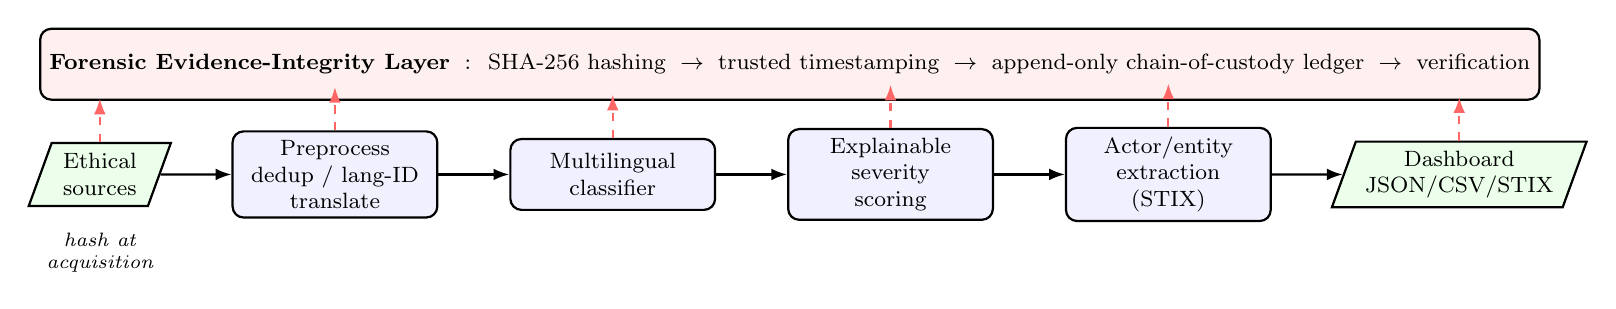
\begin{tikzpicture}[
  font=\footnotesize,
  node distance=6mm and 9mm,
  stage/.style={rectangle,rounded corners,draw,thick,align=center,
                minimum height=9mm,minimum width=26mm,fill=blue!6},
  integ/.style={rectangle,rounded corners,draw,thick,align=center,
                minimum height=9mm,minimum width=120mm,fill=red!6},
  io/.style={trapezium,trapezium left angle=70,trapezium right angle=110,
             draw,thick,align=center,fill=green!8,minimum height=8mm},
  arr/.style={-{Latex[length=2mm]},thick}
]
% top: integrity spine
\node[integ] (coc) {\textbf{Forensic Evidence-Integrity Layer} \;:\; SHA-256 hashing $\;\to\;$ trusted timestamping $\;\to\;$ append-only chain-of-custody ledger $\;\to\;$ verification};
% pipeline row
\node[io,below=14mm of coc.west,anchor=west] (src) {Ethical\\sources};
\node[stage,right=of src] (pre) {Preprocess\\dedup / lang-ID\\translate};
\node[stage,right=of pre] (cls) {Multilingual\\classifier};
\node[stage,right=of cls] (sev) {Explainable\\severity\\scoring};
\node[stage,right=of sev] (ner) {Actor/entity\\extraction\\(STIX)};
\node[io,right=of ner] (dash) {Dashboard\\JSON/CSV/STIX};
\draw[arr] (src)--(pre);
\draw[arr] (pre)--(cls);
\draw[arr] (cls)--(sev);
\draw[arr] (sev)--(ner);
\draw[arr] (ner)--(dash);
% integrity hooks
\foreach \n in {src,pre,cls,sev,ner,dash}{
  \draw[arr,red!60,dashed] (\n.north) -- ++(0,0.55);
}
\node[align=center,below=2mm of src,font=\scriptsize\itshape] {hash at\\acquisition};
\end{tikzpicture}
\caption{\framework{} architecture. A linear analytic pipeline (bottom) runs beneath a
cross-cutting evidence-integrity spine (top): every artifact entering or leaving any
stage is hashed and recorded in the chain-of-custody ledger, so analysis never breaks
provenance.}
\label{fig:arch}
\end{figure}

The architecture (Fig.~\ref{fig:arch}) deliberately renders the integrity layer as a
\emph{cross-cutting spine} rather than a terminal step: hashing and custody logging hook
into the input and output of every analytic stage. This is the structural expression of
the paper's central claim---that forensic soundness must be a property of the whole
pipeline, not an afterthought appended to its output.

%=====================================================================
\section{Dataset Strategy}\label{sec:data}

Because primary dark-web collection raises legal and ethical constraints
(Section~\ref{sec:ethics}), \framework{} is designed for a \emph{layered, reproducible}
dataset strategy that prioritizes sanitized and archival sources:

\begin{enumerate}[leftmargin=1.5em]
  \item \textbf{Archival/sanitized dark-web corpora:} publicly released darknet-market
  and forum archives used in prior peer-reviewed work (e.g., Agora-derived listings and
  forum datasets)~\cite{sangher2023towards}, with PII removed and access controlled.
  \item \textbf{Public CTI corpora for extraction:} STIX-aligned NER datasets
  (APTNER, DNRTI, CyNER-family, CyberNER) for the actor/entity
  component~\cite{wang2022aptner,evangelatos2021ner,echchammakhy2025cyberner,feng2025promptbart}.
  \item \textbf{Multilingual augmentation:} parallel/translated subsets and
  low-resource crime-text corpora to build the non-English evaluation
  sets~\cite{alharbi2025bert,nazir2025multilingual}, covering English, Hindi, Arabic,
  Russian, and French/German.
  \item \textbf{Annotation protocol:} a documented, inter-annotator-agreement-measured
  scheme for threat type and severity band, following the rigorous human-annotation
  practice reported for dark-web data~\cite{sangher2023towards}.
\end{enumerate}

\noindent\textbf{Reproducibility.} We will publish dataset construction scripts, splits,
hashes of each release, and a datasheet; raw illicit content is never redistributed,
only derived features and labels where licensing permits.

%=====================================================================
\section{Models to Compare}\label{sec:models}

Table~\ref{tab:models} lists the comparison matrix spanning classical, deep, and
transformer baselines for the classification and severity tasks.

\begin{table}[t]
\centering
\caption{Model comparison matrix. The same splits and metrics are used throughout; LLM
baselines are evaluated zero-/few-shot.}
\label{tab:models}
\small
\begin{tabular}{@{}p{3.1cm}p{4.0cm}p{5.4cm}@{}}
\toprule
\textbf{Family} & \textbf{Models} & \textbf{Role in study} \\
\midrule
Classical ML & TF-IDF $+$ LR / SVM / RF / XGBoost & Lower-bound baselines; fast, interpretable reference \\
Deep (non-transformer) & CNN, BiLSTM, BiLSTM-CRF & Sequence baselines; CRF variant for NER~\cite{kim2020automatic} \\
Monolingual transformer & BERT / RoBERTa (per language) & Per-language upper bound~\cite{sangher2023towards} \\
Multilingual transformer & mBERT, \textbf{XLM-R} & Core classifier; cross-lingual transfer~\cite{conneau2020xlmr,thangaraj2024crosslingual} \\
Generative / LLM & instruction-tuned LLM (zero/few-shot) & Modern baseline; taxonomy/extraction~\cite{shah2025madcti,demarcos2026llm,sorokoletova2024scalable} \\
NER / extraction & transformer-NER, PROMPT-BART & STIX-aligned actor/entity extraction~\cite{evangelatos2021ner,feng2025promptbart,echchammakhy2025cyberner} \\
Severity head & hybrid (posterior $+$ features) & Proposed; vs.\ classifier-confidence and CVSS-style baselines~\cite{zeng2022licality,saklani2025severity} \\
\bottomrule
\end{tabular}
\end{table}

%=====================================================================
\section{Evaluation Metrics}\label{sec:metrics}

Evaluation is multi-axis (Table~\ref{tab:metrics}), reflecting the framework's
integrated nature: a system that classifies well but explains poorly, or preserves
evidence but mis-ranks severity, fails its purpose.

\begin{table}[t]
\centering
\caption{Multi-axis evaluation metric suite.}
\label{tab:metrics}
\small
\begin{tabular}{@{}p{3.2cm}p{8.8cm}@{}}
\toprule
\textbf{Axis} & \textbf{Metrics} \\
\midrule
Classification & Accuracy, macro-/weighted-F1, precision/recall, per-class F1, MCC \\
Cross-lingual & Per-language F1; transfer gap $\Delta$F1 (zero-/few-shot vs.\ monolingual); macro-F1 across languages \\
Severity scoring & Ranking: NDCG@$k$, Spearman $\rho$ vs.\ analyst ranking; Calibration: ECE, Brier score, reliability diagrams \\
Explanation quality & Fidelity (perturbation/deletion AOPC), stability/robustness, sparsity/complexity, SHAP--LIME agreement~\cite{kalakoti2025evaluating,salih2023perspective} \\
Extraction (NER) & Entity-level F1 (STIX types), relation accuracy~\cite{wang2022aptner,echchammakhy2025cyberner} \\
Evidence integrity & Tamper-detection rate, false-accept rate, verification latency, custody-log completeness~\cite{lone2019forensicchain} \\
Efficiency & Throughput (docs/s), per-stage latency, integrity overhead (\%) \\
\bottomrule
\end{tabular}
\end{table}

%=====================================================================
\section{Evidence Integrity Validation Method}\label{sec:integrity}

The integrity layer provides a tamper-evident, auditable record for every artifact.

\paragraph{Hashing.} On acquisition, each artifact $a$ (raw or derived) is reduced to a
digest $h(a)=\text{SHA-256}(a)$. Derived artifacts additionally store the hash of their
parent, forming a hash-linked provenance DAG that mirrors the analytic transformations.

\paragraph{Timestamping.} Each digest is bound to a trusted timestamp $t$ (RFC~3161-style
TSA token or equivalent trusted time source), establishing \emph{existence-at-time} and
ordering, which is essential for evidentiary claims about collection time.

\paragraph{Chain of custody.} Custody events (collect, transform, classify, score,
export, access) are written to an append-only, hash-chained ledger: block $b_i$ stores
$\{h(a_i), t_i, \text{actor}, \text{action}, h(b_{i-1})\}$, so block $i$ commits to all
prior blocks. This yields the tamper-resistance property exploited by blockchain-based
custody schemes~\cite{lone2019forensicchain,ali2022procedure,loffi2025management}, while
remaining deployable as a lightweight permissioned ledger (no public blockchain
required). Large payloads are stored off-ledger with only their hashes
on-ledger~\cite{loffi2025management}.

\paragraph{Verification and validation.} Integrity is verified by recomputing $h(a)$ and
checking it against the ledger, and by validating the hash-chain linkage end to end. We
evaluate the layer with an adversarial \emph{tamper test}: a controlled set of
post-hoc modifications (bit-flips, substitutions, deletions, reordering, log edits) is
injected, and we report tamper-detection rate (target $100\%$), false-accept rate
(target $0\%$), and verification latency. We also report custody-log completeness and
the throughput overhead the layer imposes (RQ4).

%=====================================================================
\section{Ethical and Legal Considerations}\label{sec:ethics}

Dark-web research carries real ethical and legal risk; \framework{} is governed by an
explicit protocol. (1)~\textbf{Lawful sourcing:} preference for archived, sanitized, and
public CTI data; any live monitoring occurs only under institutional/ethics-board
approval and applicable law, and never involves participation in, solicitation of, or
payment for illegal activity. (2)~\textbf{Minimization and PII handling:} personal data
is minimized, redacted, or pseudonymized; victim data is never re-published.
(3)~\textbf{No operational uplift:} the framework is designed to detect and document
threats, not to reproduce attack capability; exploit content is handled as evidence, not
executed. (4)~\textbf{Dual-use and disclosure:} findings of imminent harm are routed to
appropriate authorities/CERTs through a responsible-disclosure process. (5)~\textbf{Legal
defensibility:} the integrity layer (Section~\ref{sec:integrity}) and explanation layer
exist partly to satisfy evidentiary and accountability standards, aligning with
forensic-readiness guidance~\cite{nist80086,lone2019forensicchain}. (6)~\textbf{Researcher
safety and access control:} collection runs in isolated environments with strict access
control and audit logging. A full ethics statement and data-management plan accompany the
paper.

%=====================================================================
\section{Ablation Study Design}\label{sec:ablation}

To establish that integration---not any single module---is the contribution (RQ5), we
ablate each component and measure the effect on end-to-end, investigator-relevant
performance (Table~\ref{tab:ablation}).

\begin{table}[t]
\centering
\caption{Ablation design. Each row removes/alters one capability; we report the change
on the most affected axis. (Cells to be filled from experiments.)}
\label{tab:ablation}
\small
\begin{tabular}{@{}p{5.4cm}p{4.0cm}cc@{}}
\toprule
\textbf{Configuration} & \textbf{Primary axis affected} & \textbf{Macro-F1} & \textbf{$\Delta$} \\
\midrule
Full \framework{} (all components) & --- & \emph{0.9X} & --- \\
$-$ multilingual (English-only model) & cross-lingual F1 & \emph{0.XX} & \emph{$-$} \\
\;translate-then-classify vs.\ native & cross-lingual F1 & \emph{0.XX} & \emph{$-$} \\
$-$ hybrid features (posterior only) & severity calibration (ECE) & \emph{0.XX} & \emph{$-$} \\
$-$ explanation layer & analyst trust / fidelity & \emph{n/a} & \emph{$-$} \\
\;SHAP only / LIME only / attention only & explanation fidelity & \emph{0.XX} & \emph{$-$} \\
$-$ integrity layer & tamper-detection rate & \emph{0\%} & \emph{$-$} \\
$-$ STIX extraction (no link analysis) & actor-recall / usability & \emph{0.XX} & \emph{$-$} \\
\bottomrule
\end{tabular}
\end{table}

%=====================================================================
\section{Expected Results}\label{sec:results}

Tables~\ref{tab:main} and~\ref{tab:lang} give the result-table \emph{templates}; values
are placeholders to be populated from experiments. We frame expectations as hypotheses
(H), to be confirmed or refuted: \textbf{H1}---a multilingual encoder closes most of the
gap to per-language monolingual models, with a bounded zero-shot transfer penalty;
\textbf{H2}---hybrid severity scoring is better calibrated (lower ECE) and better ranked
(higher NDCG) than classifier confidence; \textbf{H3}---SHAP and attention provide higher
fidelity than LIME on text, but combining them aids analyst interpretation;
\textbf{H4}---the integrity layer achieves $100\%$ tamper detection at low ($<$10\%)
throughput overhead.

\begin{table}[t]
\centering
\caption{Main classification results (template). To be completed from experiments.}
\label{tab:main}
\small
\begin{tabular}{@{}lccccc@{}}
\toprule
\textbf{Model} & \textbf{Acc.} & \textbf{Macro-F1} & \textbf{Prec.} & \textbf{Rec.} & \textbf{MCC} \\
\midrule
TF-IDF $+$ SVM      & 0.XX & 0.XX & 0.XX & 0.XX & 0.XX \\
BiLSTM              & 0.XX & 0.XX & 0.XX & 0.XX & 0.XX \\
mBERT               & 0.XX & 0.XX & 0.XX & 0.XX & 0.XX \\
XLM-R (ours, joint) & \textbf{0.9X} & \textbf{0.9X} & \textbf{0.9X} & \textbf{0.9X} & \textbf{0.XX} \\
LLM (few-shot)      & 0.XX & 0.XX & 0.XX & 0.XX & 0.XX \\
\bottomrule
\end{tabular}
\end{table}

\begin{table}[t]
\centering
\caption{Per-language and transfer results (template).}
\label{tab:lang}
\small
\begin{tabular}{@{}lccccc@{}}
\toprule
\textbf{Setting} & \textbf{EN} & \textbf{HI} & \textbf{AR} & \textbf{RU} & \textbf{FR/DE} \\
\midrule
Monolingual (F1)        & 0.XX & 0.XX & 0.XX & 0.XX & 0.XX \\
Joint multilingual (F1) & 0.XX & 0.XX & 0.XX & 0.XX & 0.XX \\
Zero-shot transfer (F1) & 0.XX & 0.XX & 0.XX & 0.XX & 0.XX \\
$\Delta$F1 (transfer gap) & --- & $-$0.0X & $-$0.0X & $-$0.0X & $-$0.0X \\
\bottomrule
\end{tabular}
\end{table}

%=====================================================================
\section{Limitations and Future Work}\label{sec:limits}

\paragraph{Limitations.} (1)~Reliance on archival/sanitized corpora may underrepresent
the most recent, ephemeral threats; live coverage is constrained by ethics and law.
(2)~Severity labels are partly subjective; inter-annotator agreement bounds the ceiling
of calibration claims. (3)~Machine translation can distort low-resource semantics and
thereby explanations, an effect we measure but cannot fully eliminate. (4)~The
permissioned-ledger integrity model resists tampering but assumes trusted timestamping
infrastructure and does not by itself prevent collection-time fabrication.
(5)~Adversaries may adapt (obfuscation, code-switching, slang) to evade detection.

\paragraph{Future work.} Extend coverage to additional low-resource and code-mixed
languages; incorporate multimodal evidence (images, marketplace screenshots); replace
post-hoc explanation with inherently interpretable severity models and evaluate analyst
trust in a user study; explore zero-knowledge proofs and self-sovereign identity for
privacy-preserving, cross-jurisdiction custody~\cite{loffi2025management}; and validate
end-to-end admissibility with legal-domain experts.

%=====================================================================
\section{Conclusion}\label{sec:conclusion}

We presented \framework{}, a framework that unifies multilingual dark-web threat
classification, explainable and calibrated severity scoring, STIX-aligned actor/entity
extraction, and a cryptographic forensic evidence-integrity layer into a single
investigator-ready pipeline. The contribution is the \emph{integration}: by making
forensic soundness and explanation cross-cutting properties of a multilingual analytic
pipeline---rather than separate, after-the-fact concerns---\framework{} produces threat
intelligence that is simultaneously multilingual, transparent, severity-aware, and
admissible. We formalized the design, specified a reproducible dataset and multi-axis
evaluation strategy, and laid out an ablation methodology to demonstrate that the
integrated whole exceeds its parts. Completing the empirical evaluation is the immediate
next step.

%=====================================================================
\section*{Paper Outline (for authors)}\label{sec:outline}
\addcontentsline{toc}{section}{Paper Outline}
\noindent
1.~Introduction (\S\ref{sec:intro}) ---
2.~Gap, Problem, Objectives, RQs (\S\ref{sec:gap}) ---
3.~Related Work, 5 themes (\S\ref{sec:related}) ---
4.~Methodology (\S\ref{sec:methodology}) ---
5.~Architecture (\S\ref{sec:architecture}) ---
6.~Dataset Strategy (\S\ref{sec:data}) ---
7.~Models Compared (\S\ref{sec:models}) ---
8.~Metrics (\S\ref{sec:metrics}) ---
9.~Evidence Integrity (\S\ref{sec:integrity}) ---
10.~Ethics \& Legal (\S\ref{sec:ethics}) ---
11.~Ablation Design (\S\ref{sec:ablation}) ---
12.~Expected Results (\S\ref{sec:results}) ---
13.~Limitations \& Future Work (\S\ref{sec:limits}) ---
14.~Conclusion (\S\ref{sec:conclusion}).

%=====================================================================
\bibliographystyle{plain}
\bibliography{references}

\end{document}
